% !TEX encoding = UTF-8
% !TEX TS-program = pdflatex
% !TEX root = ../tesi.tex

%**************************************************************
\chapter{Descrizione dello stage}
\label{cap:descrizione-stage}
%**************************************************************

\intro{In questo capitolo verrà descritto in dettaglio l'idea dello stage, l'azienda dove è stato svolto e come è stato organizzato il lavoro.}

%**************************************************************

\section{L'azienda}

\subsection{La storia}

Sync Lab S.r.l. è un'azienda di consulenza informatica nata nel 2002 nella sede di Napoli e trasformatasi molto velocemente nel corso degli anni in \textit{System Integrator} grazie ad un processo di maturazione delle competenze tecnologiche.\\ L'azienda supporta le esigenze di innovazione dei clienti offrendo soluzioni IT in ambito \textit{Business Consultancy}, \textit{Project Financing} e \textit{IT Consultancy}.\\
\begin{figure}[H]
	\begin{center}
		
\includegraphics[width=0.5\columnwidth]{logo_large}
		\caption{Logo di Sync Lab}
	\end{center}
\end{figure}
Ad oggi l'azienda conta un organico di circa 200 dipendenti ed è riuscita a coprire tutto il territorio nazionale fino ad ottenere un totale di cinque sedi a Roma, Napoli, Verona, Padova e Milano. L'azienda propone sul mercato prodotti software ed attraverso essi ha gradualmente conquistato significativamente fette di mercato nei seguenti settori: mobile, videosorveglianza e sicurezza delle infrastrutture informatiche aziendali.\\
Il loro obiettivo é quello di supportare il cliente nella Realizzazione, Messa in Opera e \textit{Governance} di soluzioni IT, sia dal punto di vista Tecnologico, sia nel Governo del Cambiamento Organizzativo.

\subsection{I prodotti}

I prodotti offerti più noti dell'azienda sono i seguenti:
\begin{itemize}
	\item \textbf{SynClinic}: sistema informativo sanitario per la gestione dei processi clinici ed amministrativi di ospedali, cliniche e case di cura. Lo scopo è diventare uno strumento indispensabile di supporto per il personale nella gestione del rischio clinico di ogni paziente;
	\item \textbf{DPS4}: web application per gestire gli adempimenti della privacy GDPR, acronimo per \textit{General Data Protection Regulation}, con lo scopo di rafforzare la privacy dei dati dei cittadini;
	\item \textbf{StreamLog}: sistema in grado di effettuare in modo semplice ed efficacie il controllo degli accessi degli utenti ai sistemi;
	\item \textbf{StreamCrusher}: software in grado di analizzare i dati che aiuta ad essere informati adeguatamente su quando bisogna prendere decisioni di business, ad identificare criticità e riorganizzare il sistema;
	\item \textbf{Wave}: acronimo per \textit{Wide Area Videosurveillance Environment}, è un prodotto software nato per ottenere un'integrazione sinergica tra i mondi della sorveglianza e dei Sistemi Informativi Territoriali (GIS) in modo da ottenere una copertura totale del territorio;
	\item \textbf{Seastream}: piattaforma in grado di migliorare la sicurezza, l'efficienza e il processo di innovazione in campo marittimo.
\end{itemize}

%**************************************************************
\section{L'idea dello stage}

\begin{figure}[H]
	\begin{center}
		
\includegraphics[width=0.5\columnwidth]{NFTLab}
		\caption{Logo di NFTLab}
	\end{center}
\end{figure}

Il progetto da svolgere proposto dall'azienda per lo stage è una web application chiamata NFTLab legata all'ambito blockchain e \gls{NFTg}. Nonostante siano due argomenti nati qualche anno fa, in questo ultimo anno la loro popolarità crebbe in maniera esponenziale e questo porta ad avere un argomento contemporaneo ed interessante per il progetto di stage.\\
All'interno della web application l'utente può navigare nella pagina principale e visualizzare le opere multimediali poste in vendita, eseguire l'accesso se possiede un account nel sito oppure registrarsi come nuovo account.\\
Dopo essere acceduto al sito, l'utente può modificare i propri dati, inserire una nuova opera multimediale o modificare i dati di quelle precedentemente inserite e comprare un'opera multimediale caricata nel sito da un altro utente.\\
Essendo un progetto legato al concetto di blockchain e \gls{NFT} le azioni di compravendita verranno effettuate tramite lo scambio di una moneta virtuale detta Ethereum. Un utente viene identificato tramite l'indirizzo del wallet con cui acquisterà o caricherà una nuova opera multimendiale.\\
Quando un utente carica un'opera multimediale, il file viene salvato tramite codice hash nella blockchain ed in questo modo le opere caricate saranno univoche. Infatti salvando queste informazioni nella blockchain viene creato un timestamp che funge da certificato di attribuzione dell'opera all'utente che carica o compra l'opera multimediale. In questo modo nessuno nessun altro utente può registrare la stessa opera a suo nome poichè una funzione hash produce sempre e solo un risultato rendendo uniche le opere multimediali.\\
Per realizzare questi aspetti sono state implementate diverse maschere, ovvero interfacce utente, tramite il framework Vue.js, uno strumento utile allo sviluppo di web application reattive e a pagina singola.\\
Parte del percorso di stage è stata riservata ad un periodo di studio delle tecnologie utili allo sviluppo delle maschere e legate al back end, in particolare è stato studiato il framework Spring. FRASE CHE NON MI PIACE

%**************************************************************
\section{Organizzazione del lavoro}

\subsection{Modello di sviluppo}

L'azienda adotta il modello di sviluppo Agile che si basa sull'interazione continua con gli \gls{stakeholderg}$_G$ e predilige:
\begin{itemize}
	\item gli individui e le loro interazioni piuttosto che i processi e gli strumenti;
	\item il software funzionante piuttosto che una documentazione esaustiva;
	\item la collaborazione con il cliente piuttosto che la negoziazione dei contratti;
	\item essere propositivi verso il cambiamento piuttosto che rifiutarlo.
\end{itemize}
L'idea di questo modello non si basa quindi su uno sviluppo sequenziale ma sul concetto di rivedere di continuo le specifiche adeguandole durante l'avanzamento dello sviluppo software. In questo modo si possono apportare agilmente modifiche mediante metodologie iterative ed incrementali con un continuo scambio di pareri ed informazioni tra gli sviluppatori ed il committente. Il progetto di stage è stato portato avanti utilizzando il metodo \gls{scrumg}$_G$.\\
Scrum è il metodo più diffuso e prevede di dividere il progetto in blocchi di lavoro detti sprint, alla fine dei quali si crea un incremento del prodotto software. Esso prevede vari meeting per controllare il lavoro svolto ed organizzare il lavoro da svolgere nel prossimo periodo. Inoltre nel corso dello sviluppo l'azienda organizza diversi meeting con gli \gls{stakeholderg} e i membri del progetto per valutare l'andamento dello sprint.\\
Gli incontri legati a questo modello di sviluppo che vengono svolti di solito sono:
\begin{itemize}
	\item sprint planning meeting: tenuto ad inizio sprint per poter organizzare il lavoro;
	\item daily scrum: riunione giornaliera del team di sviluppo per monitorare l'andamento dello sprint;
	\item sprint review: tenuto a fine sprint per valutare i risultati ottenuti e quali cambiamenti apportare per lo sprint successivo.
\end{itemize}
\begin{figure}[H]
	\begin{center}
		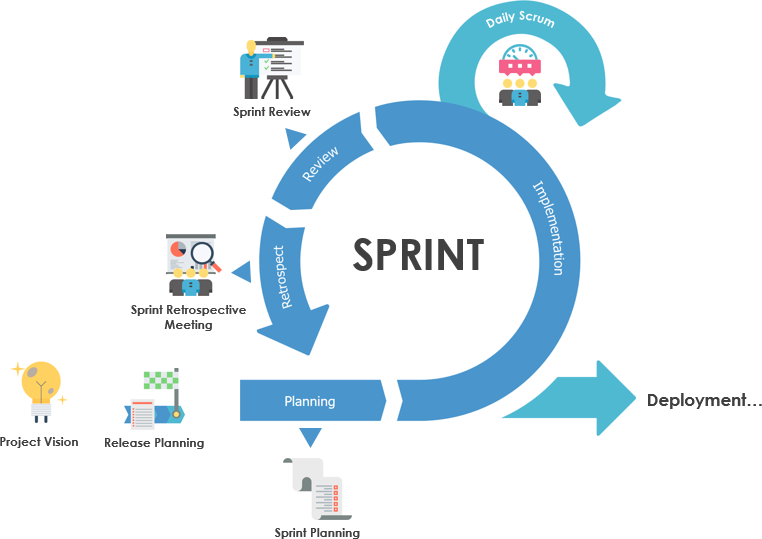
\includegraphics[width=0.5\columnwidth]{scrum}
		\caption{Metodo Scrum}
	\end{center}
\end{figure}
La situazione di emergenza sanitaria ancora non conclusa mi ha portato a vivere un'esperienza lavorativa diversa dai colleghi degli anni precedenti, infatti ha fatto sì che lo stage fosse organizzato in modalità mista: in parte da remoto ed in parte in azienda (di solito uno o due giorni alla settimana). A causa di ciò non ho potuto vivere appieno questo modello di sviluppo vista l'impossibilità di essere sempre presente in azienda. Per questo motivo il giorno concordato con i colleghi stagisti ed il tutor aziendale per andare in azienda è stato sfruttato per fare un daily scrum alternativo data la sua cadenza settimanale.\\ 
Nonostante l'emergenza sanitaria ancora in corso ho potuto comunque constatare l’efficacia e la funzionalità di questo modello di sviluppo, soprattutto per un progetto software in evoluzione quale è stato quello a cui ho lavorato.\\

\subsection{Strumenti per l'organizzazione e la comunicazione}

\subsubsection{Trello}

Trello è una piattaforma online tramite la quale si può gestire i progetti in modo semplice, gratuito e flessibile. Questa piattaforma risulta essere molto utile per l'organizzazione e la gestione del workflow online.\\
Tramite questa piattaforma è possibile rappresentare le attività da svolgere in schede inserite sotto apposite colonne di avanzamento. In base a quanto si è riusciti a realizzare, è possibile spostare manualmente o automaticamente lo stato di avanzamento di ogni scheda. Le diciture più comuni delle colonne utilizzate nella piattaforma sono le seguenti:
\begin{itemize}
	\item \textbf{attività}: elenco di schede della attività da svolgere nel corso del progetto;
	\item \textbf{in corso}: elenco di schede delle attività in corso di sviluppo;
	\item \textbf{in verifica}: elenco di schede delle attività in corso di verifica;
	\item \textbf{concluse}: elenco di schede delle attività concluse.
\end{itemize}
Per ogni scheda inoltre è possibile chi svolgerà quell'attività, commenti relativi ad essa, link ad informazioni utili per il suo svolgimento ed un elenco puntato rappresentante delle sotto-attività da compiere per il corretto svolgimento dell'attività.\\
Proprio per i numerosi vantaggi offerti dalla piattaforma l'azienda ha deciso di utilizzarla creando due bacheche:
\begin{itemize}
	\item \textbf{bacheca personale} disponibile solo allo stagista ed al tutor aziendale, dove sono stati inseriti i compiti decisi nel piano di lavoro suddivisi per settimana;
	\item\textbf{ bacheca collettiva}: disponibile a tutti gli stagisti che lavorano allo stesso progetto e ai loro rispettivi tutor aziendali, dove sono state inserite le prime idee e funzionalità legate al progetto.
\end{itemize}
Nella bacheca personale sono presenti diverse schede di numero pari alle settimane di stage da svolgere mentre nella bacheca collettiva il numero delle schede dipende dal numero di funzionalità e servizi da sviluppare. 

\subsubsection{Report giornaliero}
L'azienda ha deciso inoltre di far scrivere ad ogni stagista un file Excel su Drive come report giornaliero delle attività svolte. Grazie ad esso il tutor poteva monitorare lo stagista anche da remoto nei giorni in cui non era richiesta la presenza in azienda. Il report è suddiviso in quattro colonne:
\begin{itemize}
	\item \textbf{giorno}: indica la data in è stata fatta un'attività in formato AAAA-MM-GG, in ordine cronologico dal giorno di inizio al giorno di fine stage;
	\item \textbf{descrizione}: breve descrizione dell'attività svolta dal tirocinante compilata solitamente alla fine di ogni giornata lavorativa;
	\item \textbf{nota}: campo dove il tutor aziendale può aggiungere note di consiglio riguardo all'attività svolta come suggerimenti sugli argomenti da leggere o link a siti utili, inoltre in questo campo viene specificato quando cadono i giorni festivi;
	\item \textbf{spunta}: casella di spunta dove il tutor indica di aver visionato l'attività svolta.
\end{itemize}

\begin{figure}[H]
	\begin{center}
		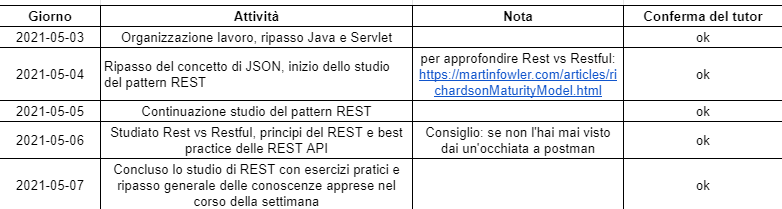
\includegraphics[width=1\columnwidth]{report}
		\caption{Spezzone del report giornaliero}
	\end{center}
\end{figure}

%**************************************************************

\subsubsection{Discord}
Discord è una piattaforma gratuita per la comunicazione dove è possibile utilizzare canali sia testuali, per lo scambio di messaggi, che vocali, per effettuare delle chiamate.\\
Per comunicare con l'intero gruppo di stagisti l'azienda ha proposto di utilizzare questa piattaforma dove noi stagisti potevamo comunicare sia con il personale aziendale che singolarmente con il proprio tutor per consigli, delucidazioni o motivi organizzativi.

\subsubsection{Notion}
Notion è un'applicazione che fornisce elementi come note, database, bacheche kanban, wiki, calendari e promemoria. L'utente può collegare questi elementi tra di loro per creare il proprio sistema per la gestione della presa di appunti, la conoscenza, la gestione dei dati e la gestione dei progetti. Questo può essere un sistema da utilizzare da soli oppure in collaborazione.\\
L'azienda ha deciso di adottare questa applicazione per segnare le presenze in azienda in modo da potersi organizzare tra i dipendenti e noi stagisti per poter rispettare le norme vigenti sul Covid.

\section{Pianificazione del lavoro}
Come definito dal piano di lavoro, lo stage è composto da un primo periodo di studio ed approfondimento teorico dei concetti e delle tecnologie ed un secondo momento di implementazione e sviluppo. La ripartizione oraria è così definita:
\begin{table}[H]
	\renewcommand{\arraystretch}{1.6}
	\begin{tabularx}{\textwidth}{lX}
		\hline
		\textbf{Durata in ore} & \textbf{Descrizione dell'attività}\\
		\hline
		40 & Presentazione dell'ambiente di sviluppo, analisi del progetto da svolgere, verifica delle credenziali assegnate e ripasso del linguaggio Java e dei concetti Web\\
		\hline
		40 & Studio dei principi generali di Spring Core (IOC e Dependency Injection), Spring Boot e Spring Data REST \\
		\hline
		40 & Studio di Spring Data JPA e studio dei concetti generali di Blockchain, Ethereum, NFT\\
		\hline
		40 & Ripasso del linguaggio di Javascript e studio del framework Vue.js\\
		\hline
		40 & Analisi e studio del progetto NFTLab, progettazione ed implementazione della nuova maschera di login\\
		\hline
		40 & Progettazione ed implementazione della nuova maschera "Upload Opera", scrittura dei service su front end di chiamata al back end ed implementazione della maschera "Gestione Opere dell'utente"\\
		\hline
		40 & Termine delle implementazioni ed integrazione con l'applicativo\\
		\hline
		40 & Termine delle integrazioni e collaudo finale\\
		\hline
	\end{tabularx}
	\label{tab:pianificazione-del-lavoro}
	\caption{Tabella della pianificazione del lavoro}
\end{table}%

\section{Requisiti ed obiettivi}
Durante la compilazione del Piano di Lavoro, documento necessario per l'inizio dello stage, sono stati definiti degli obiettivi di raggiungimento per la conclusione dello stage.

\subsection{Notazione}
La notazione tramite la quale si farà riferimento agli obiettivi è così strutturata:
\begin{center}
	\textbf{[classificazione][numero]}
\end{center}
La descrizione del codice è la seguent:
\begin{itemize}
	\item \textbf{classificazione}: individua la classificazione del requisito e può essere:
	\begin{itemize}
		\item [O =] obbligatorio
		\item [D =] desiderabile
		\item [F =] facoltativo
	\end{itemize}
\item \textbf{numero}: coppia sequenziale di numeri identificativa del requisito.
\end{itemize}
\subsection{Obiettivi fissati}
Gli obiettivi fissati sono i seguenti:
\begin{itemize}
	\item \textbf{obbligatori}:
	\begin{itemize}
		\item \underline{O01}: Acquisizione delle tematiche sopra descritte;
		\item \underline{O02}: Capacità di raggiungere gli obiettivi richiesti in autonomia seguendo il cronoprogramma;
		\item \underline{O03}: Portare a termine le implementazioni previste con una percentuale di superamento pari all'80.
	\end{itemize}
	\item \textbf{desiderabili}:
	\begin{itemize}
		\item \underline{D01}: Portare a termine le implementazioni previste con una percentuale di superamento pari al 100.
	\end{itemize}
	\item \textbf{facoltativi}:
	\begin{itemize}
		\item \underline{F01}: Riuscire a studiare e prevedere nell'implementazione la gestione del JWT Token durnate la navigazione all'interno della web app.
	\end{itemize}
\end{itemize}